\documentclass[]{article}
\usepackage{lmodern}
\usepackage{amssymb,amsmath}
\usepackage{ifxetex,ifluatex}
\usepackage{fixltx2e} % provides \textsubscript
\ifnum 0\ifxetex 1\fi\ifluatex 1\fi=0 % if pdftex
  \usepackage[T1]{fontenc}
  \usepackage[utf8]{inputenc}
\else % if luatex or xelatex
  \ifxetex
    \usepackage{mathspec}
    \usepackage{xltxtra,xunicode}
  \else
    \usepackage{fontspec}
  \fi
  \defaultfontfeatures{Mapping=tex-text,Scale=MatchLowercase}
  \newcommand{\euro}{€}
\fi
% use upquote if available, for straight quotes in verbatim environments
\IfFileExists{upquote.sty}{\usepackage{upquote}}{}
% use microtype if available
\IfFileExists{microtype.sty}{%
\usepackage{microtype}
\UseMicrotypeSet[protrusion]{basicmath} % disable protrusion for tt fonts
}{}
\ifxetex
  \usepackage[setpagesize=false, % page size defined by xetex
              unicode=false, % unicode breaks when used with xetex
              xetex]{hyperref}
\else
  \usepackage[unicode=true]{hyperref}
\fi
\hypersetup{breaklinks=true,
            bookmarks=true,
            pdfauthor={},
            pdftitle={},
            colorlinks=true,
            citecolor=blue,
            urlcolor=blue,
            linkcolor=magenta,
            pdfborder={0 0 0}}
\urlstyle{same}  % don't use monospace font for urls
\usepackage{color}
\usepackage{fancyvrb}
\newcommand{\VerbBar}{|}
\newcommand{\VERB}{\Verb[commandchars=\\\{\}]}
\DefineVerbatimEnvironment{Highlighting}{Verbatim}{commandchars=\\\{\}}
% Add ',fontsize=\small' for more characters per line
\newenvironment{Shaded}{}{}
\newcommand{\KeywordTok}[1]{\textcolor[rgb]{0.00,0.44,0.13}{\textbf{{#1}}}}
\newcommand{\DataTypeTok}[1]{\textcolor[rgb]{0.56,0.13,0.00}{{#1}}}
\newcommand{\DecValTok}[1]{\textcolor[rgb]{0.25,0.63,0.44}{{#1}}}
\newcommand{\BaseNTok}[1]{\textcolor[rgb]{0.25,0.63,0.44}{{#1}}}
\newcommand{\FloatTok}[1]{\textcolor[rgb]{0.25,0.63,0.44}{{#1}}}
\newcommand{\ConstantTok}[1]{\textcolor[rgb]{0.53,0.00,0.00}{{#1}}}
\newcommand{\CharTok}[1]{\textcolor[rgb]{0.25,0.44,0.63}{{#1}}}
\newcommand{\SpecialCharTok}[1]{\textcolor[rgb]{0.25,0.44,0.63}{{#1}}}
\newcommand{\StringTok}[1]{\textcolor[rgb]{0.25,0.44,0.63}{{#1}}}
\newcommand{\VerbatimStringTok}[1]{\textcolor[rgb]{0.25,0.44,0.63}{{#1}}}
\newcommand{\SpecialStringTok}[1]{\textcolor[rgb]{0.73,0.40,0.53}{{#1}}}
\newcommand{\ImportTok}[1]{{#1}}
\newcommand{\CommentTok}[1]{\textcolor[rgb]{0.38,0.63,0.69}{\textit{{#1}}}}
\newcommand{\DocumentationTok}[1]{\textcolor[rgb]{0.73,0.13,0.13}{\textit{{#1}}}}
\newcommand{\AnnotationTok}[1]{\textcolor[rgb]{0.38,0.63,0.69}{\textbf{\textit{{#1}}}}}
\newcommand{\CommentVarTok}[1]{\textcolor[rgb]{0.38,0.63,0.69}{\textbf{\textit{{#1}}}}}
\newcommand{\OtherTok}[1]{\textcolor[rgb]{0.00,0.44,0.13}{{#1}}}
\newcommand{\FunctionTok}[1]{\textcolor[rgb]{0.02,0.16,0.49}{{#1}}}
\newcommand{\VariableTok}[1]{\textcolor[rgb]{0.10,0.09,0.49}{{#1}}}
\newcommand{\ControlFlowTok}[1]{\textcolor[rgb]{0.00,0.44,0.13}{\textbf{{#1}}}}
\newcommand{\OperatorTok}[1]{\textcolor[rgb]{0.40,0.40,0.40}{{#1}}}
\newcommand{\BuiltInTok}[1]{{#1}}
\newcommand{\ExtensionTok}[1]{{#1}}
\newcommand{\PreprocessorTok}[1]{\textcolor[rgb]{0.74,0.48,0.00}{{#1}}}
\newcommand{\AttributeTok}[1]{\textcolor[rgb]{0.49,0.56,0.16}{{#1}}}
\newcommand{\RegionMarkerTok}[1]{{#1}}
\newcommand{\InformationTok}[1]{\textcolor[rgb]{0.38,0.63,0.69}{\textbf{\textit{{#1}}}}}
\newcommand{\WarningTok}[1]{\textcolor[rgb]{0.38,0.63,0.69}{\textbf{\textit{{#1}}}}}
\newcommand{\AlertTok}[1]{\textcolor[rgb]{1.00,0.00,0.00}{\textbf{{#1}}}}
\newcommand{\ErrorTok}[1]{\textcolor[rgb]{1.00,0.00,0.00}{\textbf{{#1}}}}
\newcommand{\NormalTok}[1]{{#1}}
\usepackage{graphicx,grffile}
\makeatletter
\def\maxwidth{\ifdim\Gin@nat@width>\linewidth\linewidth\else\Gin@nat@width\fi}
\def\maxheight{\ifdim\Gin@nat@height>\textheight\textheight\else\Gin@nat@height\fi}
\makeatother
% Scale images if necessary, so that they will not overflow the page
% margins by default, and it is still possible to overwrite the defaults
% using explicit options in \includegraphics[width, height, ...]{}
\setkeys{Gin}{width=\maxwidth,height=\maxheight,keepaspectratio}
\setlength{\parindent}{0pt}
\setlength{\parskip}{6pt plus 2pt minus 1pt}
\setlength{\emergencystretch}{3em}  % prevent overfull lines
\providecommand{\tightlist}{%
  \setlength{\itemsep}{0pt}\setlength{\parskip}{0pt}}
\setcounter{secnumdepth}{0}

\date{}

% Redefines (sub)paragraphs to behave more like sections
\ifx\paragraph\undefined\else
\let\oldparagraph\paragraph
\renewcommand{\paragraph}[1]{\oldparagraph{#1}\mbox{}}
\fi
\ifx\subparagraph\undefined\else
\let\oldsubparagraph\subparagraph
\renewcommand{\subparagraph}[1]{\oldsubparagraph{#1}\mbox{}}
\fi

\begin{document}
	\title{\huge\textbf{Camera Calibration}\LARGE \\Project: Marker-based Localization}
	\author{Niharika Jayanthi, Dheeraj Kamath \\Mentor: Sanam Shakya}
	\maketitle
	\pagebreak
\section{Goals}\label{goals}

\begin{itemize}
\tightlist
\item
  To understand how a camera is calibrated
\item
  Using cv2.calibrateCamera() function
\end{itemize}

\section{Theory}\label{theory}

Cheap pinhole cameras used for capturing images or videos introduce
significant distortion in them. These distortions are constants and can
be eliminated. Through calibration, one may also calculate the
relationship between image units and real world units. On calibration,
we obtain the camera matrix, which can be used later during pose
estimation.

Here, to perform calibration, we have used a chessboard. The chessboard
was shot from several different angles. A chessboard is used as it has
well-defined points. Certain specific corners in the chessboard are
detected. We obtain the image points from the picture and the
object(real world) points are already known to us.

\begin{figure}[htbp]
\centering
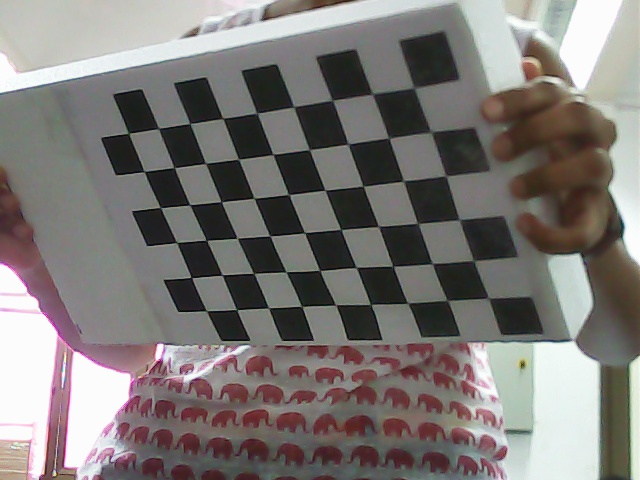
\includegraphics{images/Camera Calibration/Chessboard.jpg}
\caption{Chessboard held at an angle}
\end{figure}

\subsection{Setup}\label{setup}

You will need- 
\begin{itemize}
	\item A pinhole camera
	\item A chessboard
\end{itemize}

In the code, we will need to specify what kind of pattern we are looking
for (9x6 grid, 5x5 grid etc). As specified above, we need the object
points and their corresponding image points for calibration. It is easy
to obtain the image points from the image itself. But for the object
points, we can assume that the camera is in an XY plane, i.e.~in Z=0
plane. The camera is assumed to be moved away. So the object points can
be specified in terms of size of chessboard square. If the size of
square is 1 unit, object points can be (0,0), (1,0), (2,0)\ldots{}

\section{Code}\label{code}

The main functions used here are-

\emph{\textbf{cv2.calibrateCamera(objectPoints, imagePoints,
imageSize{[}, cameraMatrix{[}, distCoeffs{[}, rvecs{[}, tvecs{[},
flags{[}, criteria{]}{]}{]}{]}{]}{]}) → retval, cameraMatrix,
distCoeffs, rvecs, tvecs}}

where-

\begin{itemize}
\item
  \textbf{objectPoints} -- In the new interface it is a vector of
  vectors of calibration pattern points in the calibration pattern
  coordinate space. The outer vector contains as many elements as the
  number of the pattern views. If the same calibration pattern is shown
  in each view and it is fully visible, all the vectors will be the
  same. Although, it is possible to use partially occluded patterns, or
  even different patterns in different views. Then, the vectors will be
  different. The points are 3D, but since they are in a pattern
  coordinate system, then, if the rig is planar, it may make sense to
  put the model to a XY coordinate plane so that Z-coordinate of each
  input object point is 0. In the old interface all the vectors of
  object points from different views are concatenated together.
\item
  \textbf{imagePoints} -- In the new interface it is a vector of vectors
  of the projections of calibration pattern points. imagePoints.size()
  and objectPoints.size() and imagePoints{[}i{]}.size() must be equal to
  objectPoints{[}i{]}.size() for each i. In the old interface all the
  vectors of object points from different views are concatenated
  together.
\item
  \textbf{imageSize} -- Size of the image used only to initialize the
  intrinsic camera matrix.
\item
  \textbf{cameraMatrix} -- Output 3x3 floating-point camera matrix. If
  CV\_CALIB\_USE\_INTRINSIC\_GUESS and/or CV\_CALIB\_FIX\_ASPECT\_RATIO
  are specified, some or all of fx, fy, cx, cy must be initialized
  before calling the function.
\item
  \textbf{distCoeffs} -- Output vector of distortion coefficients (k\_1,
  k\_2, p\_1, p\_2{[}, k\_3{[}, k\_4, k\_5, k\_6{]}{]}) of 4, 5, or 8
  elements.
\item
  \textbf{rvecs} -- Output vector of rotation vectors (see Rodrigues() )
  estimated for each pattern view. That is, each k-th rotation vector
  together with the corresponding k-th translation vector (see the next
  output parameter description) brings the calibration pattern from the
  model coordinate space (in which object points are specified) to the
  world coordinate space, that is, a real position of the calibration
  pattern in the k-th pattern view (k=0.. M -1).
\item
  \textbf{tvecs} -- Output vector of translation vectors estimated for
  each pattern view.
\item
  \textbf{flags} -- Different flags that may be zero or a combination of
  the following values: \textbf{CV\_CALIB\_USE\_INTRINSIC\_GUESS}-
  cameraMatrix contains valid initial values of fx, fy, cx, cy that are
  optimized further. Otherwise, (cx, cy) is initially set to the image
  center ( imageSize is used), and focal distances are computed in a
  least-squares fashion. Note, that if intrinsic parameters are known,
  there is no need to use this function just to estimate extrinsic
  parameters. Use solvePnP() instead.
\end{itemize}

\textbf{CV\_CALIB\_FIX\_PRINCIPAL\_POINT}- The principal point is not
changed during the global optimization. It stays at the center or at a
different location specified when CV\_CALIB\_USE\_INTRINSIC\_GUESS is
set too.

\textbf{CV\_CALIB\_FIX\_ASPECT\_RATIO}- The functions considers only fy
as a free parameter. The ratio fx/fy stays the same as in the input
cameraMatrix . When CV\_CALIB\_USE\_INTRINSIC\_GUESS is not set, the
actual input values of fx and fy are ignored, only their ratio is
computed and used further.

\textbf{CV\_CALIB\_ZERO\_TANGENT\_DIST}- Tangential distortion
coefficients (p\_1, p\_2) are set to zeros and stay zero.
CV\_CALIB\_FIX\_K1,\ldots{},CV\_CALIB\_FIX\_K6 The corresponding radial
distortion coefficient is not changed during the optimization. If
CV\_CALIB\_USE\_INTRINSIC\_GUESS is set, the coefficient from the
supplied distCoeffs matrix is used. Otherwise, it is set to 0.

\textbf{CV\_CALIB\_RATIONAL\_MODEL}- Coefficients k4, k5, and k6 are
enabled. To provide the backward compatibility, this extra flag should
be explicitly specified to make the calibration function use the
rational model and return 8 coefficients. If the flag is not set, the
function computes and returns only 5 distortion coefficients.

\begin{itemize}
\tightlist
\item
  \textbf{criteria} -- Termination criteria for the iterative
  optimization algorithm.
\end{itemize}

\begin{center}\rule{0.5\linewidth}{\linethickness}\end{center}

\emph{\textbf{cv2.findChessboardCorners(image, patternSize{[},
corners{[}, flags{]}{]}) → retval, corners}}

where-

\textbf{image} - Source chessboard view. It must be an 8-bit grayscale
or color image.

\textbf{patternSize} - Number of inner corners per a chessboard row and
column ( patternSize = cvSize(points\_per\_row,points\_per\_colum) =
cvSize(columns,rows) ).

\textbf{corners} - Output array of detected corners.

\textbf{flags} - Various operation flags that can be zero or a
combination of the following values:

\textbf{CV\_CALIB\_CB\_ADAPTIVE\_THRESH}- Use adaptive thresholding to
convert the image to black and white, rather than a fixed threshold
level (computed from the average image brightness).

\textbf{CV\_CALIB\_CB\_NORMALIZE\_IMAGE}- Normalize the image gamma with
equalizeHist() before applying fixed or adaptive thresholding.

\textbf{CV\_CALIB\_CB\_FILTER\_QUADS}- Use additional criteria (like
contour area, perimeter, square-like shape) to filter out false quads
extracted at the contour retrieval stage.

\textbf{CALIB\_CB\_FAST\_CHECK}- Run a fast check on the image that
looks for chessboard corners, and shortcut the call if none is found.
This can drastically speed up the call in the degenerate condition when
no chessboard is observed.

The complete code is -

\begin{Shaded}
\begin{Highlighting}[]
\CommentTok{#Imports}
\ImportTok{import} \NormalTok{cv2}
\ImportTok{import} \NormalTok{numpy }\ImportTok{as} \NormalTok{np}

\CommentTok{# Termination criteria}
\NormalTok{criteria }\OperatorTok{=} \NormalTok{(cv2.TERM_CRITERIA_EPS }\OperatorTok{+} \NormalTok{cv2.TERM_CRITERIA_MAX_ITER, }\DecValTok{30}\NormalTok{, }\FloatTok{0.001}\NormalTok{)}

\CommentTok{# Define object points for a 9x6 grid}
\NormalTok{objp }\OperatorTok{=} \NormalTok{np.zeros((}\DecValTok{6}\OperatorTok{*}\DecValTok{9}\NormalTok{,}\DecValTok{3}\NormalTok{), np.float32)}
\NormalTok{objp[:,:}\DecValTok{2}\NormalTok{] }\OperatorTok{=} \NormalTok{np.mgrid[}\DecValTok{0}\NormalTok{:}\DecValTok{9}\NormalTok{,}\DecValTok{0}\NormalTok{:}\DecValTok{6}\NormalTok{].T.reshape(}\OperatorTok{-}\DecValTok{1}\NormalTok{,}\DecValTok{2}\NormalTok{)}
\NormalTok{objp }\OperatorTok{=} \NormalTok{objp }\OperatorTok{*} \DecValTok{26}

\CommentTok{# Arrays to store object points and image points}
\NormalTok{objpoints }\OperatorTok{=} \NormalTok{[] }\CommentTok{# 3d point in real world space}
\NormalTok{imgpoints }\OperatorTok{=} \NormalTok{[] }\CommentTok{# 2d points in image plane.}

\NormalTok{vd }\OperatorTok{=} \NormalTok{cv2.VideoCapture(}\DecValTok{0}\NormalTok{)}

\ControlFlowTok{while}\NormalTok{(}\VariableTok{True}\NormalTok{):}

    \NormalTok{ret, img }\OperatorTok{=} \NormalTok{vd.read()}
    \NormalTok{cv2.imshow(}\StringTok{"Video cap"}\NormalTok{, img)}
   
    \NormalTok{inp }\OperatorTok{=} \NormalTok{cv2.waitKey(}\DecValTok{1}\NormalTok{)}
    
    \ControlFlowTok{if} \NormalTok{inp }\OperatorTok{==} \DecValTok{115}\NormalTok{: }\CommentTok{#If input is 's'}
        \NormalTok{gray }\OperatorTok{=} \NormalTok{cv2.cvtColor(img,cv2.COLOR_BGR2GRAY)}

        \CommentTok{# Find the chess board corners}
        \NormalTok{ret, corners }\OperatorTok{=} \NormalTok{cv2.findChessboardCorners(gray, (}\DecValTok{9}\NormalTok{,}\DecValTok{6}\NormalTok{), }\VariableTok{None}\NormalTok{)}

        \CommentTok{# If found, add object points and image points}
        \ControlFlowTok{if} \NormalTok{ret }\OperatorTok{==} \VariableTok{True}\NormalTok{:}
            \NormalTok{objpoints.append(objp)}

            \CommentTok{#Refine image points}
            \NormalTok{cv2.cornerSubPix(gray,corners,(}\DecValTok{11}\NormalTok{,}\DecValTok{11}\NormalTok{),(}\OperatorTok{-}\DecValTok{1}\NormalTok{,}\OperatorTok{-}\DecValTok{1}\NormalTok{),criteria)}
            \NormalTok{imgpoints.append(corners)}

            \CommentTok{# Draw and display the corners}
            \NormalTok{cv2.drawChessboardCorners(img, (}\DecValTok{9}\NormalTok{,}\DecValTok{6}\NormalTok{), corners, ret)}
            \ControlFlowTok{if} \NormalTok{ret }\OperatorTok{==} \VariableTok{True}\NormalTok{:}
                \NormalTok{cv2.imshow(}\StringTok{'img'}\NormalTok{,img)}
                \NormalTok{cv2.waitKey(}\DecValTok{500}\NormalTok{)}

    \ControlFlowTok{elif} \NormalTok{inp }\OperatorTok{==} \DecValTok{27}\NormalTok{: }\ControlFlowTok{break}


\NormalTok{ret, mtx, dist, rvecs, tvecs }\OperatorTok{=} \NormalTok{cv2.calibrateCamera(objpoints,}
                                                   \NormalTok{imgpoints, gray.shape[::}\OperatorTok{-}\DecValTok{1}\NormalTok{],}
                                                   \VariableTok{None}\NormalTok{,}\VariableTok{None}\NormalTok{)}



\BuiltInTok{print} \StringTok{"Camera calibration matrix}\CharTok{\textbackslash{}n\textbackslash{}n}\StringTok{"}\NormalTok{, mtx}

\CommentTok{#Save camera matrix and distortion coefficients to be used later}
\NormalTok{np.save(}\StringTok{'cam_broke_mtx'}\NormalTok{, mtx)}
\NormalTok{np.save(}\StringTok{'cam_broke_dist'}\NormalTok{, dist)}

\NormalTok{cv2.destroyAllWindows()}
\end{Highlighting}
\end{Shaded}

\section{Resources}\label{resources}

\begin{itemize}
\tightlist
\item
  http://docs.opencv.org/2.4.1/modules/calib3d/doc/camera\_calibration\_and\_3d\_reconstruction.html
\item
  https://www.ics.uci.edu/\textasciitilde{}majumder/vispercep/cameracalib.pdf
\item
  http://homepages.inf.ed.ac.uk/rbf/CVonline/LOCAL\_COPIES/EPSRC\_SSAZ/node5.html
\item
  http://docs.opencv.org/doc/tutorials/calib3d/camera\_calibration/camera\_calibration.html
\item
  http://opencv-python-tutroals.readthedocs.org/en/latest/py\_tutorials/py\_calib3d/py\_calibration/py\_calibration.html\#calibration
\end{itemize}

\section{Exercises}\label{exercises}

\begin{itemize}
\tightlist
\item
  Try to calibrate different cameras.
\item
  Try using different patterns to detect.
\end{itemize}

\end{document}
